\chapter{KI ilegal nutzen?}
Zuerst dachte ich, dass es gar nicht so viele Optionen geben kann KI ilegal zu nutzen, denn es ist doch hauptsächlich ein Hilfsmittel.
Später kam mir dann der Gedanke wie es denn mit Gesichtserkennung und ständiger überwachung aussieht. Dies sollte jedoch gar nicht wirklich ilegal sein. 
Ich lag jedoch auf der richtigen Spur, denn das ilegalste was man mit KI tun kann ist: Deepfake.
Deepfakes sind realistisch wirkende Medieninhalte, die durch Techniken der künstlichen Intelligenz abgeändert, erzeugt, also verfälscht worden sind.\citep{deepfake-wikipedia}
Deepfake wird fast überall angewendet. Jedoch hauptsächlich bei:
\begin{itemize}
    \item Politik
    \item Kunst
    \item Datenschutz
    \item Forschung
    \item Pornografie
\end{itemize}
Diese neue Kunst der Manipulation bringt natürlich gewaltige Probleme mit sich, z.B. kann man nun eigentlich keinen Medien mehr glauben schenken, oder sobald man sein Gesicht irgendwo gepostet hat kann es für Pornografie oder anderes ausgenutzt werden.
Speziell schlimm finde ich jedoch gefälschte Anrufe, also wenn man anhand einer auch nur noch so kurzen Sprachdatei eine eigene KI trainiert, welche genau so spricht wie diese Person. Dies ist auch eine grosse Betrugsmasche auf welche besonders ätere Personen reinfallen. Man muss jedoch aufpassen, denn wenn die ganzen KI's sich mit einer solchen geschwindigkeit weiterentwickeln können selbst gut informierte bald nicht mehr zwischen echt und generiert unterscheiden.
Unter folgendem Link könnt ihr eure eigen Stimmbot trainieren oder Stimmen von Olaf Scholz, Angela Merkel, usw. verwenden \href{https://de.vidnoz.com/stimme-klonen.html?insur=degooglecamp_voiceclone_stimmen%20ai%20eigene%20stimme&gad_source=1&gclid=CjwKCAjwx-CyBhAqEiwAeOcTdXzrCxZKDQlEb6uY7WpuKmMl4A4Kjq1nL8A8dgPwKI11yVB6GCWjixoCfvIQAvD_BwE}{vidnoz.com}.
Was momentan noch wegen witzig verwendet wird kann auch ganz anderst verwendet werden und es ist nicht einmal schwer.
Auch habe ich da gerade erst einen Spendenaufruf einer Nachbarin herumeilte überlegt ob nicht auch dies komplett ausgenutzt werden wird.
\clearpage
Ursprünglich dachte ich dies könne noch lange nicht passieren da alle KI generierten Bilder die ich kenne so aussehen:
\begin{figure}[H]
    \centering
    
\includegraphics[width=0.5\textwidth]{copilot(dall-e)2.jpeg}
    \caption{Bild erstellt mit Copilot von Bing, also Dall-e}-
    \label{fig:copilot(dall-e)}
\end{figure}

Nun habe ich jedoch nach etwas recherche \href{https://this-person-does-not-exist.com}{diese} Webseite gefunden und hier sind extrem realistische KI Bilder von Menschen zu finden.
\begin{figure}[H]
    \centering
    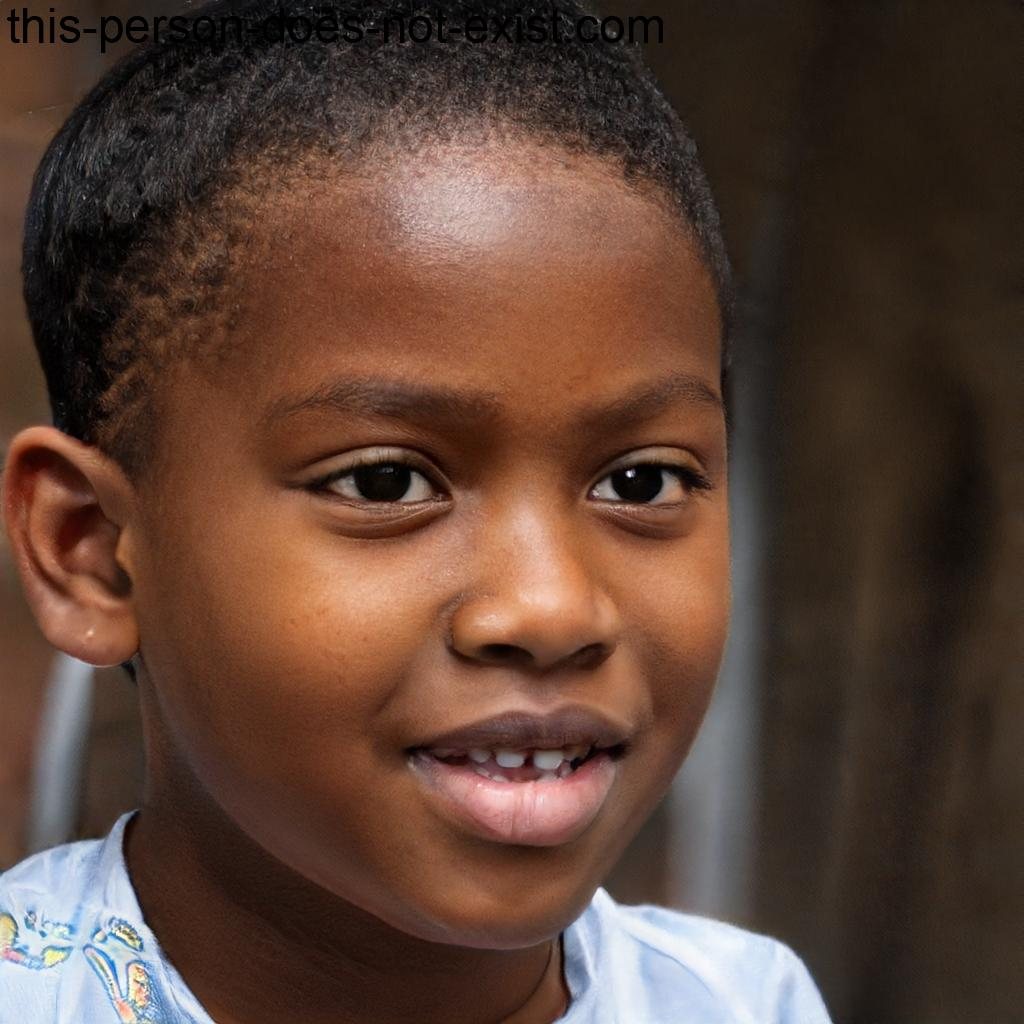
\includegraphics[width=0.5\textwidth]{this_person_does_not_exist2.jpeg}
    \caption{Bild von der Webseite \href{https://this-person-does-not-exist.com}{this-person-does-not-exist.com}.}
    \label{fig:this_person_does_not_exist}
\end{figure}
Manche Bilder kann man mit Hilfe der Tipps welche unten bei der Webseite stehen noch von echten Bildern unterscheiden. Bei so vielen geht es jedoch schon nicht mehr. Dies schockte mich. Ein solches Bild kann man für 15\$ von ihnen abkaufen, was nicht viel ist wenn man bedenkt, dass man damit mehrere tausend Leute hineinlegen kann und um Spendengeld betrügen kann.
\section{Fazit}

Auch hier komme ich zur Schlussfolgerung, dass der ethische Aspekt im Umgang mit KI erneut bei dem Menschen liegt. Jedoch finde ich nun, dass es nicht nur noch an dem Ersteller liegt und wie stark er das Ganze einschränkt sonder, auch wie der Nutzer das Ganze nutzt.
Also all das Deepfakezeug muss ja nicht unbedingt negativ genutzt werden, es kann auch in einem lustigen Sinn verwendet werden, z.B. seine Freunde "never gonna let you down" singen zu lassen.
Auch spielt es meiner Meinung nun mehr eine Rolle was der Nutzer denn überhaupt möchte, denn nur das wird vom Ersteller erstellt.